\documentclass[Thesis.tex]{subfiles}
\begin{document}

\chapter{Variational Description}

\section{Variational principles for discrete metrics in $\mathbb{E}^2$, $\mathbb{H}^2$, and $\mathbb{S}^2$}

Construction of discrete flat metrics. A discrete Euclidean flat metric is the minimizer of a convex functional.
\begin{eqnarray}
\lambda_{ij} &:=& 2\log l_{ij}\\
\tilde\lambda_{ij} &:=& \lambda_{ij}+u_i+u_j\\
f_{Euc}(u_i, u_j, u_k) &:=& \alpha_i \tilde \lambda_{jk} + \alpha_j \tilde \lambda_{ki} + \alpha_k \tilde \lambda_{ij} + 2\left(\ML(\alpha_i) + \ML(\alpha_j) + \ML(\alpha_k)\right)
\end{eqnarray}

\begin{definition}
\begin{eqnarray}
	E_{Euc}(u) &:=& \sum_{ijk\in F}\left(f_{Euc}(u_i, u_j, u_k) - \frac{\pi}{2}\left(\tilde \lambda_{jk} + \tilde \lambda_{ki} + \tilde \lambda_{ij}\right)\right) + \sum_{i\in V} \Theta_i u_i
\end{eqnarray}
\end{definition}

 This definition and the derivatives can be found in \cite{Bobenko2010}

For the hyperbolic case $\lambda$ and $\tilde\lambda$ are defined as before. Further define
\begin{eqnarray}
	\beta_i &:=& \frac{1}{2} \left(\pi + \alpha_i - \alpha_j - \alpha_k \right)\\
	\beta_j &:=& \frac{1}{2} \left(\pi - \alpha_i + \alpha_j - \alpha_k \right)\\
	\beta_k &:=& \frac{1}{2} \left(\pi - \alpha_i - \alpha_j + \alpha_k \right)\\
	f_{Hyp}(u_i, u_j, u_k) &:=&\beta_i \tilde \lambda_{jk} + \beta_j \tilde \lambda_{ki} + \beta_k \tilde \lambda_{ij}\\ 		
				&&+\ML(\alpha_i) + \ML(\alpha_j) + \ML(\alpha_k) + \ML(\beta_i) + \ML(\beta_j) + \ML(\beta_k)\\
				&&+\ML\left(\frac{1}{2} (\pi - \alpha_i - \alpha_j - \alpha_k)\right)
\end{eqnarray}

\begin{definition}
\begin{eqnarray}
	E_{Hyp}(u) &:=& \sum_{ijk\in F}\left(f_{Hyp}(u_i, u_j, u_k) - \frac{\pi}{2}\left(\tilde \lambda_{jk} + \tilde \lambda_{ki} + \tilde \lambda_{ij}\right)\right) + \sum_{i\in V} \Theta_i u_i
\end{eqnarray}
\end{definition}


\section{Quotient spaces and fundamental domains}

Every Riemann surface $R$ has a universal cover $X$, i.e., a simply connected covering space and a corresponding covering map. A metric of constant curvature on a compact $2$-manifold can be realized as the quotient of the universal cover over a uniformizing group.

Triangulated surfaces of genus $g\geq 2$ without boundary can be equipped with a discretely conformally equivalent flat hyperbolic metric \cite{Bobenko2010}. By flat hyperbolic metric we mean that the edge length are hyperbolic and for any vertex the angle sum is $2\pi$. To realize this metric in the hyperbolic plane e.g. in the Poicar\'e disk model one has to introduce cuts along a basis of the homotopy. This creates a simply connected domain in $\mathbb H^2$. Matching cut paths are realated by a hyperbolic motion i.e. the M\"obius transformations that leave the unit disk invariant (Figure~\ref{fig:axes_of_motion}).

\subsection{The cut-graph and fuchsian groups}
\emph{Want so say here: the number of transformations generated by the mapping of corresponding edges equals the number of path segments in the homotopy-cut-graph. They generate a fuchsian group with \#vertices relations}


\begin{figure}
\centering
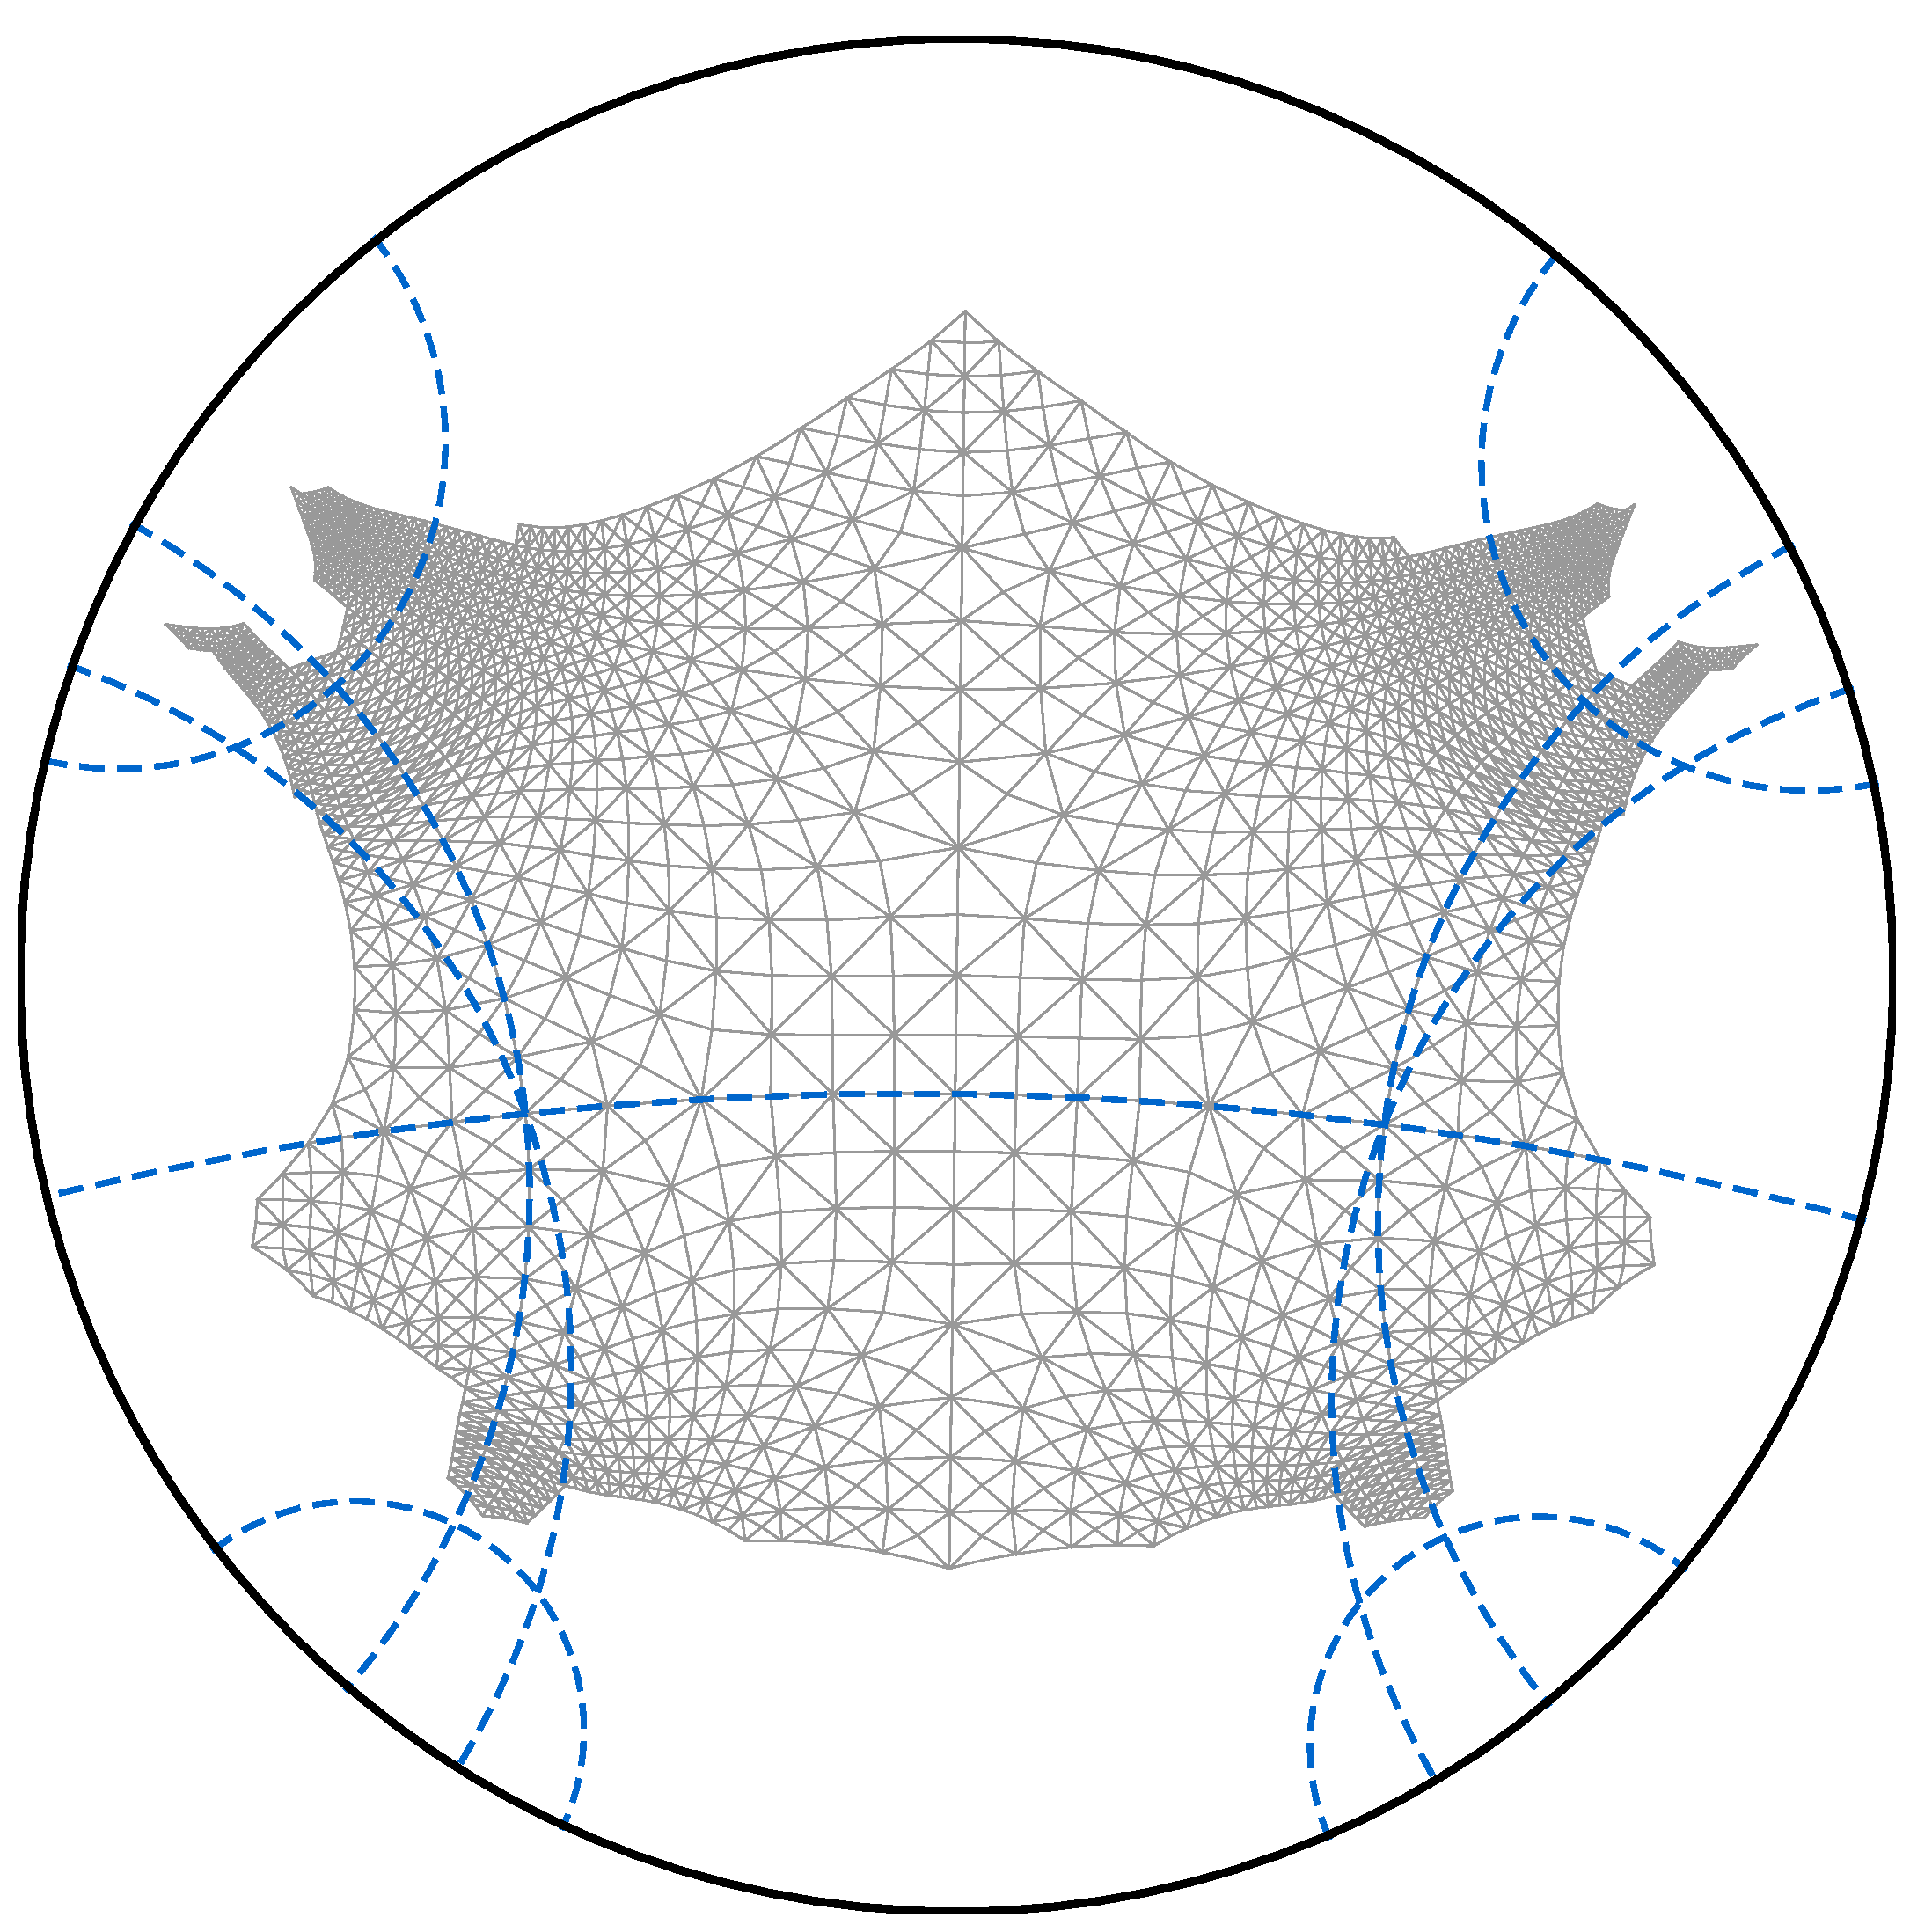
\includegraphics[width=0.4\linewidth]{cutCuttedBrezel01}
\caption{Hyperbolic flat metric on a genus $2$ surface and the axes of the associated hyperbolic motions.}
\label{fig:axes_of_motion}
\end{figure}

\subsection{Minimal presentation}
\subsection{Separated handles}
\subsection{Opposite sides identified}
\subsection{Canonical Keen Polygons}

\section{Uniformization of embedded genus $g=0$, $g=1$, and $g>1$ surfaces}

\subfilebibliography
\end{document}

%%% Local Variables:
%%% TeX-master: "Thesis.tex"
%%% End: